\documentclass[a4paper]{article}

\title{Machine Learning Engineer Nanodegree}
\author{Daniel Valcarce}
\usepackage{hyperref}
\usepackage{xcolor}
\usepackage{array}
\usepackage{graphicx}
\usepackage{subcaption}
\usepackage{float}
\hypersetup{colorlinks,linkcolor={red!50!black}, citecolor={blue!50!black}, urlcolor={blue!80!black}}

\renewcommand{\thesection}{\Roman{section}} 
\renewcommand{\thesubsection}

\graphicspath{{images/}}

\begin{document}
	\pagenumbering{gobble}
	\maketitle
	\newpage
	\pagenumbering{arabic}
	
	\section{Definition}
	\subsection{Project Overview}
	According to the World malaria report \footnote{\label{malaria_report}\url{https://www.who.int/malaria/media/world-malaria-report-2018/en/}} , in 2017, an estimated 219 million cases of malaria
	occurred worldwide (95\% confidence interval [CI]: 203–262 million), compared with 239
	million cases in 2010 (95\% CI: 219–285 million) and 217 million cases in 2016 (95\% CI: 200–259
	million).
	
	\medskip
	In 2017, there were an estimated 435 000 deaths from malaria globally, compared with
	451000 estimated deaths in 2016, and 607000 in 2010. Nearly 80\% of global malaria deaths in
	2017 were concentrated in 17 countries in the WHO African Region and India; 7 of these
	countries accounted for 53\% of all global malaria deaths.

	\subsection{Problem Statement}
	In order to reduce the burden for microscopists in resource-constrained regions and improve
	diagnostic accuracy, the \textit{National Library of Medicine}\footnote{\label{nlm_web}\url{https://www.nlm.nih.gov/}} provide us with a dataset\footnote{\label{dataset}\url{https://ceb.nlm.nih.gov/proj/malaria/cell_images.zip}} with which I
	will create a model to detect malaria parasite in thin blood smear images.
	
	\medskip
	A common approach to create similar models consist in resize the images to a common size in order to train the model, then use this model to predict and classify new images. In this project I will apply a technique called \textbf{Progressive resizing} which consist of training different models for different size of images.
	
	\medskip
	The idea behind this technique is to create different models for different image sizes. First I need to decide which sizes could be good to train the model based on the data exploration, then I'll create and train a model with the images resized to the lower size I chose. Once the first model is trained, I will apply transfer learning to create and train the second model with the next size for the images, and so on with all chosen sizes.
	
	\medskip
	For each model I will obtain different metrics in order to know which model performs better and also to know if this technique is useful for this dataset.
	
	\subsection{Metrics}
	This project is based on the research article \textit{"Pre-trained convolutional neural networks as feature extractors toward improved malaria parasite detection in thin blood smear images"}\footnote{\label{research_paper}\url{https://www.ncbi.nlm.nih.gov/pmc/articles/PMC5907772/}} where Dr Rajaraman S and his
	team shown a table\footnote{\label{table_metrics}\url{https://www.ncbi.nlm.nih.gov/pmc/articles/PMC5907772/table/table-6/}} with the performance metrics results obtained during their experiments,
	comparing their custom model against other well-known models like AlexNet, VGG-16,
	ResNet-50, Xception and DenseNet-121.
	
	\medskip
	For this project I will use the same metrics and then compare the results against the values of
	their custom model.		
	
	\begin{table}[h!]
		\begin{center}
			\caption{Metrics}
			{\renewcommand{\arraystretch}{2}%
			\begin{tabular}{l|c}
				\textbf{Name} & \textbf{Formula} \\
				\hline
				Accuracy & $ \frac{TP + TN}{TP + TN + FP + FN} $ \\
				AUC & formula \\
				Sensitivity & $ \frac{TP}{TP + FN} $ \\
				Specificity & $ \frac{TN}{TN + FP} $ \\
				F1-score & $ \frac{2TP}{2TP + FP + FN} $ \\
				MCC & $ \frac{TP \times TN - FP \times FN}{\sqrt{(TP + FP)(TP + FN)(TN + FP)(TN + FN)}} $ \\
			\end{tabular}} \quad
		\end{center}
	\end{table}

	\medskip
	\begin{itemize}
		\item TP: True Positives
		\item TN: True Negatives
		\item FP: False Positives
		\item FN: False Negatives
	\end{itemize}
	

\newpage

	\section{Analysis}
	\subsection{Data Exploration}	
	The dataset contains a total of 27558 color images separated in two folders, Parasitized folder and
	Uninfected folder with 13779 images each.
	
	\medskip
	The images were manually annotated by an expert slide reader at the Mahidol-Oxford Tropical Medicine Research Unit in Bangkok, Thailand.
	
	\medskip
	The image sizes varies between 49x58 and 349x241 pixels.
	
	\begin{figure}[h!]
		\centering
		\begin{subfigure}[b]{0.4\linewidth}
			\centering
			\captionsetup{justification=centering}
			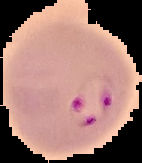
\includegraphics[width=3cm, height=3cm]{parasitized.png}
			\caption{Parasitized cell}
		\end{subfigure}\quad
		\begin{subfigure}[b]{0.4\linewidth}
			\centering
			\captionsetup{justification=centering}
			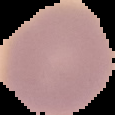
\includegraphics[width=3cm, height=3cm]{uninfected.png}
			\caption{Uninfected cell}
		\end{subfigure}
		\caption{Dataset sample}
		\label{fig:cells}
	\end{figure}

	\subsection{Exploratory Visualization}
	The plots below show how is the distribution of images regarding of it size in order to select the best values to apply the progressive resizing technique.
	
	\medskip
	The Figures 2 and 3 show us that the X values (width) are between 120 and 145 for most of the images with only a few outliers.

	
	\begin{figure}[H]
		\centering
		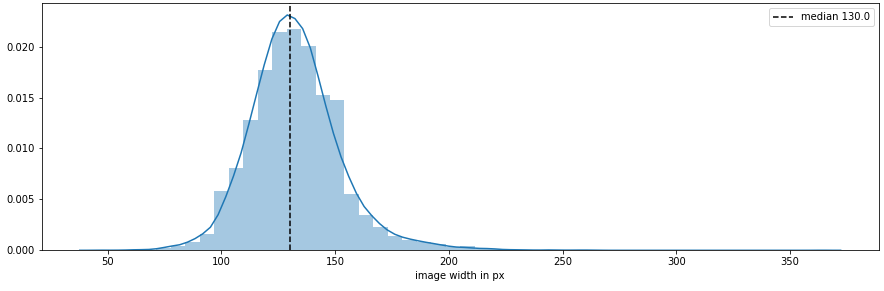
\includegraphics[width=.9\textwidth]{dist_x.png}
		\caption{Distribution chart based on the image width}
		\label{fig:width_dist}
	\end{figure}
	\begin{figure}[H]
		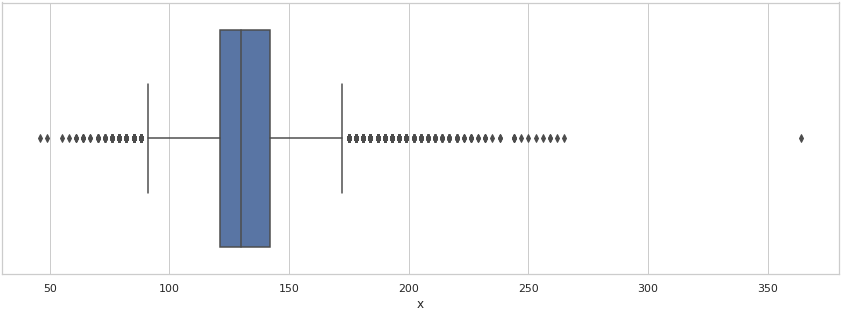
\includegraphics[width=.9\textwidth]{box_x.png}
		\caption{Box chart based on the image width}
		\label{fig:width_box}
	\end{figure}

	\medskip
	The Figures 4 and 5 show how is the distribution for the  Y values (height) and looks similar to the X values, this means that the images are almost square images therefore there will be not much distortion when I will apply the resizing during the training process.
	
	\begin{figure}[H]
		\centering
		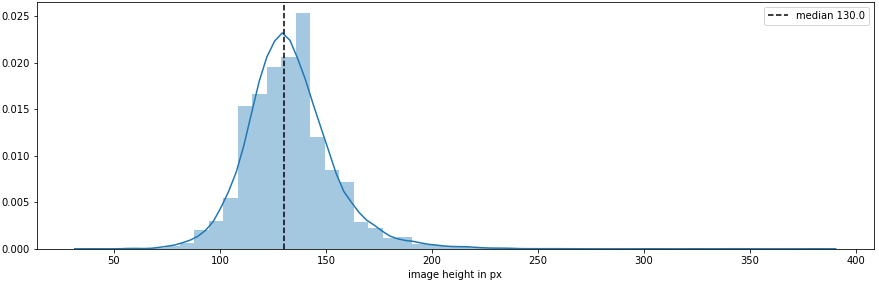
\includegraphics[width=.9\textwidth]{dist_y.png}
		\caption{Distribution chart based on the image height}
		\label{fig:height_dist}
	\end{figure}
	\begin{figure}[H]
		\centering
		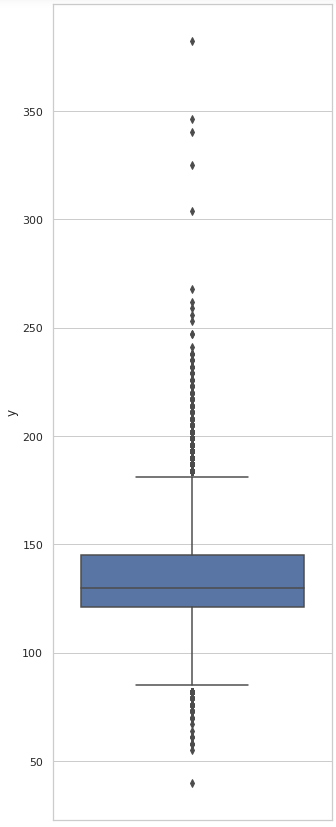
\includegraphics[width=.5\textwidth]{box_y.png}
		\caption{Distribution based on the image height}
		\label{fig:height_box}
	\end{figure}

	\medskip
	The Table 2 shows the size for images with min/max values for each property, X and Y.

	\medskip
	\begin{table}[h!]
		\centering
		\caption{Min/Max mesures}
		\label{tab:minmax}
		\begin{tabular}{l|c|c}
			\textbf{} & {X} & {Y} \\
			\hline
			Max X & 364 & 340 \\
			Max Y & 208 & 382 \\
			Min X & 46 & 79 \\
			Min Y & 55 & 40 \\
		\end{tabular}
	\end{table}

	\subsection{Algorithms and Techniques}
	
	\subsection{Benchmark}
	
	\section{Methodology}
	
	\subsection{Data Preprocesing}
	
	\subsection{Implementation}
	
	\subsection{Refinement}
	
	\section{Results}
	
	\subsection{Model Evaluation and Validation}
	
	\subsection{Justification}
	
	\section{Conclusion}
	
	\subsection{Free-Form Visualization}
	
	\subsection{Reflection}
	
	\subsection{Improvement}
	
\end{document}